\documentclass[12pt, letterpaper]{article}
\usepackage[letterpaper, portrait, margin=1in]{geometry}   %For page Setup
\usepackage[utf8]{inputenc}
\usepackage{amssymb, amsmath}               %For Equations and Formulas
\usepackage{comment}                        %For Commenting
\usepackage{hyperref}                       %For Hyperlinks
\usepackage{listings}                       %For Coding Examples
\usepackage[table]{xcolor}                  %For Coloring Tables
\usepackage{xcolor}                         %For Color Associated with Coding Examples
\usepackage{multicol}                       %For Making Multiple Columns
\usepackage{multirow}                       %Allows for multiple cells in one row in a table
\usepackage{graphicx, epstopdf}                       %Converts eps files to pdf
\usepackage{textcomp}                       %For the Copyright and Registered Rights Symbols
\epstopdfsetup{update}

\title{PIC10F200 Reference}
\author{K}
\date{June 3, 2020}

\usepackage{natbib}
\usepackage{graphicx}

\hypersetup{                                %Setup for Hyperlink Colors
    colorlinks=true,
    linkcolor=blue,                         %For Hyperlinked Text
    filecolor=magenta,                      %For Text that Hyperlinks to other Files
    urlcolor=cyan,                          %For Hyperlinked Printed URLs
}



\begin{document}

\begin{comment}
\begin{titlepage}
    %\titlepage
    \maketitle
\end{titlepage}
\end{comment}

\maketitle

\tableofcontents{}
\pagebreak

\section{PIC10F200 Datasheet}
Here is a link to the \href{https://ww1.microchip.com/downloads/en/DeviceDoc/40001239F.pdf}{PIC10F200 Datasheet}.

\noindent \textbf{Table of Contents}

\renewcommand{\labelenumii}{\arabic{enumii}}          %This uses aribic numbers for the second level
\begin{enumerate}

  % Section 1
  \item General Description (Page 4)
  \begin{enumerate}
    \item [1.1] Applications (Page 4)
  \end{enumerate}

  % Section 2
  \item PIC10F200/202/204/206 Device Varieties (Page 5)
  \begin{enumerate}
    \item [2.1] Quick Turn Programming (QTP) Devices (Page 5)
    \item [2.2] Serialized Quick Turn Programming$^\text{SM}$ (SQTP$^\text{SM}$) Devices (Page 5)
  \end{enumerate}

  % Section 3
  \item Architectual Overview (Page 6)
  \begin{enumerate}
    \item [3.1] Clock Scheme/Instruction Cycle (Page 10)
    \item [3.2] Instruction Flow/Pipelining (Page 10)
  \end{enumerate}

  % Section 4
  \item Memory Organization (Page 11)
  \begin{enumerate}
    \item [4.1] Program Memory Organization for the PIC10F200/204 (Page 11)
    \item [4.2] Program Memory Organization for the PIC10F202/206 (Page 12)
    \item [4.3] Data Memory Organization (Page 12)
    \begin{enumerate}
      \item [4.3.1] GENERAL PURPOSE REGISTER FILE (Page 12)
      \item [4.3.2] SPECIAL FUNCTION REGISTERS (Page 14)
    \end{enumerate}
    \item [4.4] STATUS Register (Page 15)
    \item [4.5] OPTION Register (Page 16)
    \item [4.6] OSCCAL Register (Page 17)
    \item [4.7] Program counter (Page 18)
    \begin{enumerate}
      \item [4.7.1] EFFECTS OF RESET (Page 18)
    \end{enumerate}
    \item [4.8] Stack (Page 18)
    \item [4.9] Indirect Data Addressing: INDF and FSR Registers
    \item [4.10] Indirect Addressing
  \end{enumerate}

  % Section 5
  \item I/O Port (Page 20)
  \begin{enumerate}
    \item [5.1] GPIO (Page 20)
    \item [5.2] TRIS Registers (Page 20)
    \item [5.3] I/O Interfacing (Page 20)
    \item [5.4] I/O Programming Considerations (Page 21)
    \begin{enumerate}
      \item [5.4.1] BIDIRECTIONAL I/O PORTS (Page 21)
      \item [5.4.2] SUCCESSIVE OPERATIONS ON I/O PORTS (Page 21)
    \end{enumerate}
  \end{enumerate}

  % Section 6
  \item Timer0 Module and TMR0 Register (PIC10F200/202) (Page 23)
  \begin{enumerate}
    \item [6.1] Using Timer0 with an External Clock (PIC10F200/202) (Page 24)
    \begin{enumerate}
      \item [6.1.1] EXTERNAL CLOCK SYNCRONIZATION (Page 24)
      \item [6.1.2] TIMER0 INCREMENT DELAY (Page 25)
    \end{enumerate}
    \item Prescaler (Page 25)
    \begin{enumerate}
      \item [6.2.1] SWITCHING PRESCALER ASSIGNMENT (Page 25)
    \end{enumerate}
  \end{enumerate}

  % Section 7
  \item Timer0 Module and TMR0 Register (PIC10F204/206) (Page 27)
  \begin{enumerate}
    \item [7.1] Using Timer0 with an External Clock (PIC10F204/206) (Page 28)
    \begin{enumerate}
      \item [7.1.1] EXTERNAL CLOCK SYNCRONIZATION (Page 28)
      \item [7.1.2] TIMER0 INCREMENT DELAY (Page 29)
    \end{enumerate}
    \item [7.2] Prescaler (Page 29)
    \begin{enumerate}
      \item [7.2.1] SWITCHING PRESCALER ASSIGNMENT (Page 29)
    \end{enumerate}
  \end{enumerate}

  % Section 8
  \item Comparator Module (Page 31)
  \begin{enumerate}
    \item [8.1] Comparator Configuration (Page 32)
    \item [8.2] Comparator Operation (Page 33)
    \item [8.3] Comparator Reference (Page 33)
    \item [8.4] Comparator Response Time (Page 33)
    \item [8.5] Comparator Output (Page 33)
    \item [8.6] Comparator Wake-up Flag (Page 33)
    \item [8.7] Comparator Operation During Sleep (Page 33)
    \item [8.8] Effects of a Reset (Page 33)
    \item [8.9] Analog Input Connection Considerations (Page 33)
  \end{enumerate}

  % Section 9
  \item Special Features of the CPU (Page 35)
  \begin{enumerate}
    \item [9.1] Configuration Bits (Page 35)
    \item [9.2] Oscillator Configurations (Page 36)
    \begin{enumerate}
      \item [9.2.1] OSCILLATOR TYPES (Page 36)
      \item [9.2.2] INTERNAL 4MHz OCILLATOR (Page 36)
    \end{enumerate}
    \item [9.3] Reset (Page 36)
    \begin{enumerate}
      \item [9.3.1] $\overline{\text{MCLR}}$ ENABLE (Page 37)
    \end{enumerate}
    \item [9.4] Power-on-Reset (POR) (Page 37)
    \item [9.5] Device Reset Timer (DRT) (Page 40)
    \item [9.6] Watchdog Timer (Page 40)
    \begin{enumerate}
      \item [9.6.1] WDT PERIOD
      \item [9.6.2] WDT PROGRAMMING CONSIDERATIONS
    \end{enumerate}
    \item [9.7] Time-out Sequence, Power-down and Wake-up from Sleep Status Bits ($\overline{\text{TO}}$, $\overline{\text{PD}}$, GPWUF, CWUF) (Page 42)
    \item [9.8] Reset on Brown-out (Page 42)
    \item [9.9] Power-down Mode (Sleep) (Page 43)
    \begin{enumerate}
      \item [9.9.1] SLEEP (Page 43)
      \item [9.9.2] WAKE-UP FROM SLEEP (Page 43)
    \end{enumerate}
    \item [9.10] Program Verification/Code Protection (Page 44)
    \item [9.11] ID Locations (Page 44)
    \item [9.12] In-Circuit Serial Programming$^{TM}$ (Page 44)
  \end{enumerate}

  % Section 10
  \item Instruction Set Summary (Page 45)

  % Section 11
  \item Development Support (Page 53)
  \begin{enumerate}
    \item [11.1] MPLAB X Integrated Development Environment Software (Page 53)
    \item [11.2] MPLAB XC Compilers (Page 54)
    \item [11.3] MPASM Assembler (Page 54)
    \item [11.4] MPLINK Object Linker/MPLIB Object Librarian (Page 54)
    \item [11.5] MPLAB Assembler, Linker and Librarian for Various Device Families (Page 54)
    \item [11.6] MPLAB X SIM Software Simulator (Page 55)
    \item [11.7] MPLAB REAL ICE In-Circuit Emulator System (Page 55)
    \item [11.8] MPLAB ICD 3 In-Circuit Debugger System (Page 55)
    \item [11.9] PICkit 3 In-Circuit Debugger/Programmer (Page 55)
    \item [11.10] PMLAB PM3 Device Programmer (Page 55)
    \item [11.11] Demonstration/Development Boards, Evaluation Kits, and Starter Kits (Page 56)
    \item [11.12] Third Party Development Tools (Page 56)
  \end{enumerate}

  % Section 12
  \item Electrical Characteristics (Page 57)
  \begin{enumerate}
    \item [12.1] DC Characteristics: PIC10F200/202/204/206 (Industrial) (Page 59)
    \item [12.2] DC Characteristics: PIC10F200/202/204/206 (Extended) (Page 60)
    \item [12.3] DC Characteristics: PIC10F200/202/204/206 (Industrial, Extended) (Page 61)
    \item [12.4] Timing Parameter Symbology and Load Conditions - PIC10F200/202/204/206 (Page 63)
  \end{enumerate}

  % Section 13
  \item DC and AC Characteristics Graphs and Tables (Page 67)

  % Section 14
  \item Packaging Information (Page 75)
  \begin{enumerate}
    \item [14.1] Package Marking Information (Page 75)
    \item [14.2] Package Details (Page 78)
  \end{enumerate}

  \item [] APPENDIX A: REVISION HISTORY (Page 84)
  \begin{enumerate}
    \item [] REVISION C (August 2006) (Page 84)
    \item [] REVISION D (April 2007) (Page 84)
    \item [] REVISION E (October 2013) (Page 84)
    \item [] REVISION F (September 2014) (Page 84)
  \end{enumerate}

  \item [] The Microchip Website (Page 85)

  \item [] Customer Change Notification Service (Page 85)

  \item [] Customer Support (Page 85)

  \item [] Product Identification System (Page 86)
\end{enumerate}

\section{Tutorials}
\subsection{Circuit Bread}
\subsubsection{Part 1}
\href{https://www.circuitbread.com/tutorials/how-to-use-a-simple-microcontroller-series-intro-pic10f200-part-1}{How to use a Simple Microcontroller Series Intro (PIC10F200) - Part 1}\\
\subsubsection{Part 2}
\href{https://www.circuitbread.com/tutorials/equipment-for-our-simple-microcontroller-tutorials-pic10f200-part-2}{Equiptment for our Simple Microcontroller tutorials (PIC10F200) - Part 2}\\
\subsubsection{Part 3}
\href{https://www.circuitbread.com/tutorials/microcontroller-architecture-part-3-simple-microcontroller-pic10f200}{Microcontroller Architecture - Part 3 Simple Microcontroller (PIC10F200)}\\
\subsubsection{Part 4}
\href{https://www.circuitbread.com/tutorials/circuit-setup-mplab-x-ide-part-4-simple-microcontroller-pic10f200}{Circuit Setup / MPLAB X IDE  - Part 4 Simple Microcontroller (PIC10F200)}\\
\subsubsection{Part 5}
\href{https://www.circuitbread.com/tutorials/the-first-assembly-program-part-5-simple-microcontroller-pic10f200}{The First Assembly Program - Part 5 Simple Microcontroller (PIC10F200)}\\
\subsubsection{Part 6}
\href{https://www.circuitbread.com/tutorials/how-to-blink-an-led-part-6-microcontroller-basics-pic10f200}{How to Blick an LED - Part 6 Microcontroller Basics (PIC10F200)}\\
\subsubsection{Part 7}
\href{https://www.circuitbread.com/tutorials/pwm-led-dimming-part-7-microcontroller-basics-pic10f200}{Creating a PWM in Assembly - Part 7 Microcontroller Basics (PIC10F200)}\\
\subsubsection{Part 8}
\href{https://www.circuitbread.com/tutorials/musical-microcontroller-part-8-microcontroller-basics-pic10f200}{Musical Microcontroller - Part 8 Microcontroller Baics (PIC10F200)}\\
\subsubsection{Part 9}
\href{https://www.circuitbread.com/tutorials/button-inputs-part-9-microcontroller-basics-pic10f200?token=LmskE2t7648abpBhlu5zQP1KYlriMAeo}{Button Inputs - Part 9 Microcontroller Basics (PIC10F200)}\\
\subsubsection{Special}
\href{https://www.circuitbread.com/tutorials/christmas-lights-special-microcontroller-basics-pic10f200}{Christmas Lights Special - Microcontroller Basics (PIC10F200)}\\
\subsubsection{Part 10}
\href{https://www.circuitbread.com/tutorials/servo-motor-indirect-addressing-and-electronic-lock---part-10-microcontroller-basics-pic10f200}{Servo motor, indirect addressing, and electric lock - Part 10 Microcontroller Basics (PIC10F200)}\\
\subsubsection{Part 11}
\href{https://www.circuitbread.com/tutorials/communicating-with-a-pc-using-uart---part-11-microcontroller-basics-pic10f200}{Communicating with a PC using UART - Part 11 Microcontroller Basics (PIC10F200)}\\
\subsubsection{Part 12}
\href{https://www.circuitbread.com/tutorials/bluetooth-controlled-robot?token=w_zWrzkxdM0H4BuRq-v0tg9uQv_kKaYI}{Bluetooth Controlled Robot - Part 12 Microcontroller Basics (PIC10F200)}\\
\subsubsection{Part 13}
\href{https://www.circuitbread.com/tutorials/line-following-car-part-13-microcontroller-basics-pic10f200}{Line Following Car - Part 13 Microcontroller Basics (PIC10F200)}\\
\subsubsection{Part 14}
\href{https://www.circuitbread.com/tutorials/obstacle-avoidance-robot-part-14-microcontroller-basics-pic10f200}{Obstacle Avoidance Robot - Part 14 Microcontroller Basics (PIC10F200)}\\
\subsubsection{Part 15}
\href{https://www.circuitbread.com/tutorials/i2c-fm-radio-part-15-microcontroller-basics-pic10f200}{I2C FM Radio - Part 15 Microcontroller Basics (PIC10F200)}\\
\subsubsection{Part 16}
\href{https://www.circuitbread.com/tutorials/digital-thermometer-part-16-microcontroller-basics-pic10f200}{Digital Thermometer - Part 16 Microcontroller Basics (PIC10F200)}\\
\subsubsection{Part 17}
\href{https://www.circuitbread.com/tutorials/sine-wave-generator-part-17-microcontroller-basics-pic10f200}{Sine Wave Generator - Part 17 Microcontroller Basics (PIC10F200)}\\
\subsubsection{Part 18}
\href{https://www.circuitbread.com/tutorials/digital-voltmeter-part-18-microcontroller-basics-pic10f200}{Digital Voltmeter - Part 18 Microcontroller Basics (PIC10F200)}\\
\subsubsection{Part 19}
\href{https://www.circuitbread.com/tutorials/infrared-rgb-led-controller-part-19-microcontroller-basics-pic10f200}{Infrared RGB LED controller - Part 19 Microcontroller Basics (PIC10F200)}\\
\subsubsection{Part 20}
\href{https://www.circuitbread.com/tutorials/1602-character-lcd-part-20-microcontroller-basics-pic10f200?token=he8HKfRsVXpEyyyeqTTF}{1602 Character LCD - Part 20 Microcontroller Basics (PIC10F200)}

\section{$\text{PICkit}^{\text{TM}}$ 3 Programmer/Debugger}
\subsection{$\text{PICkit}^{\text{TM}}$ 3 Programmer/Debugger Labels and Pinout}
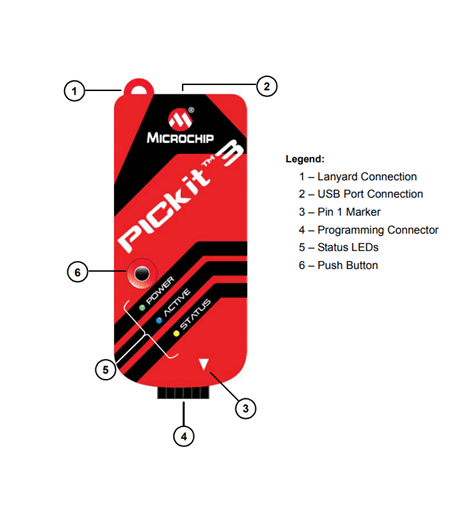
\includegraphics[scale=0.5]{Images/PICKit3 Labels}
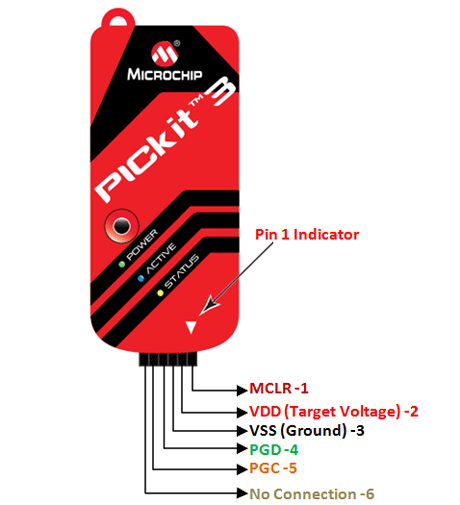
\includegraphics[scale=0.5]{Images/PICKit3 Pinout}
\subsection{$\text{PICkit}^{\text{TM}}$ 3 Programmer/Debugger User's Guide}
\url{https://ww1.microchip.com/downloads/en/DeviceDoc/51795B.pdf}
\subsection{$\text{PICkit}^{\text{TM}}$ 3 In-Circuit Debugger/Programmer User's Guide\\
For $\text{MPLAB}^{\circledR}$ X IDE}
\url{http://ww1.microchip.com/downloads/en/devicedoc/52116a.pdf}

\section{Integrated Development Environments}
\subsection{MPLAB X\textregistered \smallskip{} IDE}
MPLAB X\textregistered \smallskip{} Integrated Development Environment\\
\url{https://www.microchip.com/en-us/development-tools-tools-and-software/mplab-x-ide}

\url{https://www.microchip.com/en-us/development-tools-tools-and-software/mplab-x-ide}
\subsubsection{MPLAB Archives}
This includes archives for:
\begin{itemize}
  \item MPLAB X IDE
  \item MPLAB IDE
  \item Language Tools
  \item MPLAB C Compiler for PIC18 MCUs
  \item MPLAB C Compiler for PIC24 MCUs and dsPIC\textregistered \smallskip{} DSCs
  \item MPLAB C Compiler for PIC32 MCUs
  \item HI-TECH C Compilers
  \item Source Code
  \item $\text{PICkit}^{\text{TM}}$ Programmer/Debugger
  \item Funcitional Saftey Compilers
\end{itemize}
\url{https://www.microchip.com/en-us/development-tools-tools-and-software/mplab-ecosystem-downloads-archive}

\subsection{Manuals}
$\text{MPASM}^{\text{TM}}$ Assembler, $\text{MPLINK}^{\text{TM}}$ Object Linker, $\text{MPLIB}^{\text{TM}}$ Object Librarian User's Guide\\
\url{http://ww1.microchip.com/downloads/en/DeviceDoc/33014K.pdf}
\end{document}
